%!TEX root = ./ERL Industrial Robots.tex



%--------------------------------------------------------------------
%--------------------------------------------------------------------
\section{The \erlir Testbed at Bonn-Rhein-Sieg University of Applied Science (BRSU) - Implementation Details}
\label{ssec:IST_atHometestbed}

Based on the general design and specifications of the \erlir testbed detailed previously in this text, in this sub-section we present the exact design specifications of the \erlir testbed installed at the premises of the Bonn-Rhein-Sieg University of Applied Science (BRSU), Germany (Figure~\ref{fig:BRSU_atwork_dimension}). 

\begin{figure}[htb]
 \begin{center}
 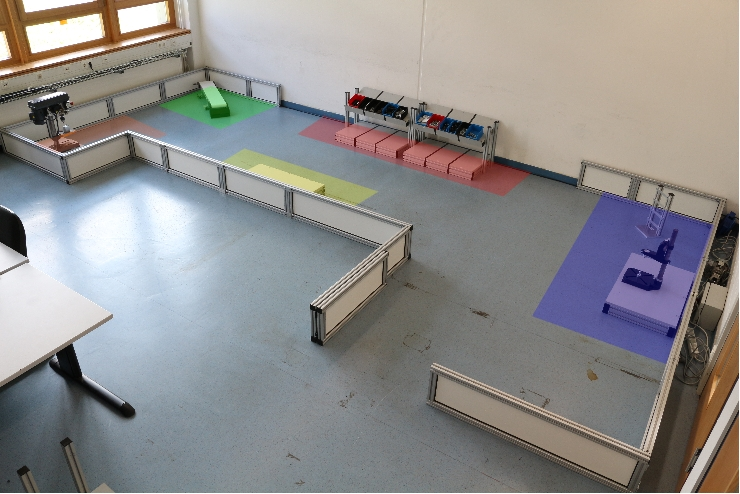
\includegraphics[width=12.5cm]{./fig/WorkArenaBRSUSpatialArea.jpg} 
 \caption{\erlir testbed at BRSU}
 \label{fig:BRSU_atwork_layout}
 
  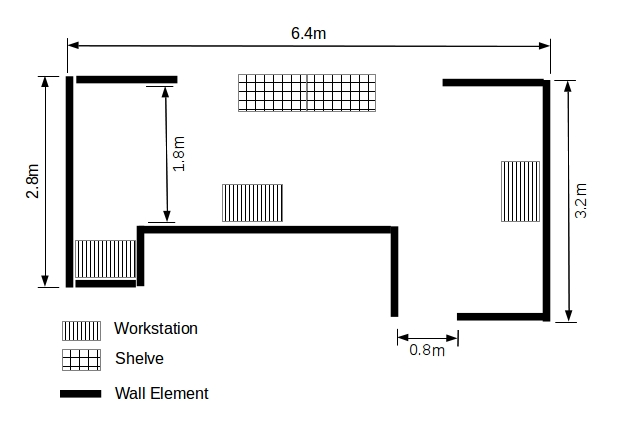
\includegraphics[width=12.5cm]{./fig/WorkArenaBRSUSpatialAreaDimension.jpg} 
 \caption{Layout of \erlir testbed at BRSU}
 \label{fig:BRSU_atwork_dimension}
 \end{center}
\end{figure}


%

Note that this \erlir testbed is not an exact replica of the actual \erlir Competition testbed but fits its general specifications and, as such, can be seen as a concrete example of using them for an actual implementation. 
More pictures of \erlir testbed are presented in Figures~\protect{\ref{fig:TaskRelatedObjects}}--\ref{fig:RoawTestBed2014}.

\subsection{Environment Structure and Properties}

\begin{itemize}
 \item Ensemble of five spatial areas which are all accessible to the robots.
 The spatial areas are shelves (red), force fitting workstation (blue), conveyor belt (green), drilling workstation (orange) and assembly workstation (yellow).
 \item Flat with no stairs.
 \item Connectivity of spatial areas:  Please refer to Figure~\ref{fig:BRSU_atwork_layout}.
 \item Sizes of spatial areas: Please refer to Figure~\ref{fig:BRSU_atwork_dimension}.
 \item Walls are mainly constructed by interconnected wall elements with a height of 30 cm.
 \item Workstations (force fitting machine, drilling machine) are elevated platform with an approximate height of 10 cm. 
 %\item Ceilings: Uniform false roof made of coated and perforated aluminum segments without slopes.
 %\item Bedroom specifications (and furniture): one open-able and tilt-able window, a double bed, two side tables, two table lamps and one large wardrobe with mirror.
 %\item Living room specification (and furniture's): contains windows that cannot be opened, couch, two armchairs, one coffee table, one TV table and one large floor lamp.
 %\item Dining room specification (and furniture's): One glass-top dining table and 2 dining chairs.
 %\item Kitchen specification (and furniture's): One kitchen table and 2 chairs, kitchen cabinet with multiple drawers and wash sink, two wall-mounted kitchen shelves.
 %\item Hallway: consists of one coat rack.
 \end{itemize}

\subsection{Objects in the Environment}

The objects in this testbed is given below through Tables~\ref{tab:TabelEnvironmentElements}~to~\ref{tab:TabelNetworkedDevices}. 
The tables are based on the arena constructed in BRSU as presented in Figure \ref{fig:BRSU_atwork_layout}.
A different arrangement as shown in Figure \ref{fig:RoawTestBed2013} or \ref{fig:RoawTestBed2014} will change the number of required items.
Environment elements (Table ~\ref{tab:TabelEnvironmentElements}) consist of walls, shelves, workstation and assembly aid tray rack.
These elements are purchased from RK Rose+Krieger GmbH company.
Networked devices (Table ~\ref{tab:TabelNetworkedDevices}) consist of quality control camera system, drilling machine, force fitting machine and central factory hub.
These equipment are custom made by the \erlir organizer.
%Benchmarking system (Table ~\ref{tab:TabelBenchmarkingSystem})  consists of the OptiTrack system, benchmarking server and benchmarking hub server.
Finally, there are also task-related objects such as motor, axis, bearing box which are already presented in the rule book.


\begin{table}[htb]
 \begin{tabular}{|p{5cm}|p{2cm}|p{5cm}|}
 \hline
 \textbf{Element} & \textbf{Quantity} & \textbf{Dimension} \\ \hline
 Wall element 80 & 10 & 80x4x30cm \\ \hline
 Wall element 120 & 10 & 120x4x30cm \\ \hline
 Wall element 54 & 10 & 54x4x30cm \\ \hline
 Assembly aid tray & 1 & 20x15x40cm \\ \hline
 Workstation & 3 & 80x50x10 cm \\ \hline
 Shelves & 4 & 1760x50x50 cm \\ \hline
\end{tabular}
\caption{Environment elements}
\label{tab:TabelEnvironmentElements}
\end{table}

\begin{figure}[htb]
 \begin{center}
 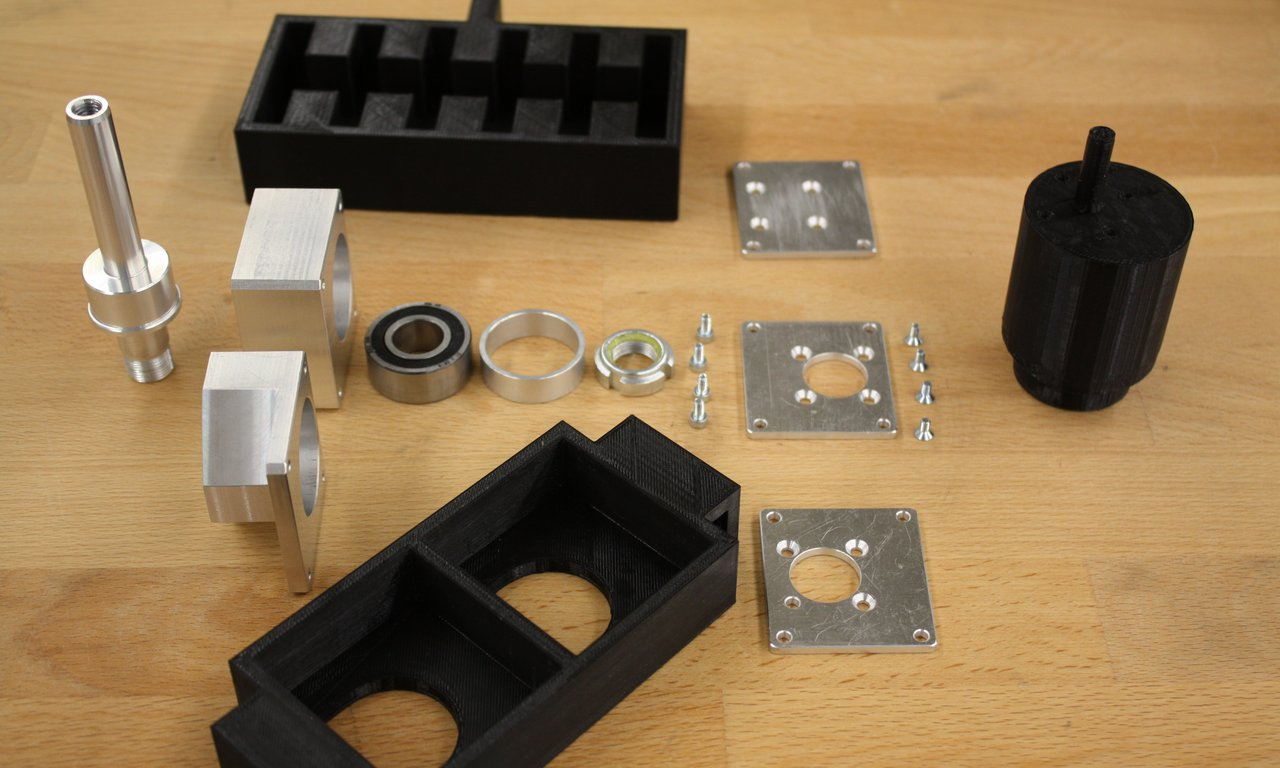
\includegraphics[width=9cm]{pics/atwork/objects/roawObjects.jpg} 
 \end{center}
 \caption{Task-related objects}
 \label{fig:TaskRelatedObjects}
\end{figure}


%\begin{table}[htb]
% \begin{tabular}{|p{10cm}|p{2cm}|}
% \hline
% \textbf{Device} & \textbf{Quantity} \\ \hline
% OptiTrack FLEX: V100 R2 Camera & 22 \\ \hline
% OptiTrack OptiHub & 4 \\ \hline
% Windows PC: motion capture software & 1 \\ \hline 
% Linux PC: ROS-based benchmarking software & 1 \\ \hline
%\end{tabular}
%\caption{Benchmarking system}
%\label{tab:TabelBenchmarkingSystem}
%\end{table}


\begin{table}[htb]
 \begin{tabular}{|p{6cm}|p{2cm}|p{6cm}|}
 \hline
 \textbf{Device} & \textbf{Quantity} & \textbf{Parts} \\ \hline
 Quality control camera system & 1 & - Microsoft HD webcam  \\ 
 & & - Conveyor belt \\
 & & - Conveyor belt motor \\ 
 & & - Raspberry Pi \\ \hline
 
 Drilling machine & 1 & - Drilling machine  \\
 & & - Maxon motor \\
 & & - Motor controller \\ 
 & & - Raspberry Pi \\ \hline
 
 Force fitting machine & 1 & - Press fit \\
 & & - Maxon motor \\
 & & - Motor controller \\ 
 & & - Raspberry Pi \\ \hline
 
 Central Factory Hub & 1 & - Linux PC \\ 
 & & - Ethernet switch \\ \hline
\end{tabular}
\caption{Networked devices}
\label{tab:TabelNetworkedDevices}
\end{table}

\begin{figure}[htb]
 \begin{center}
 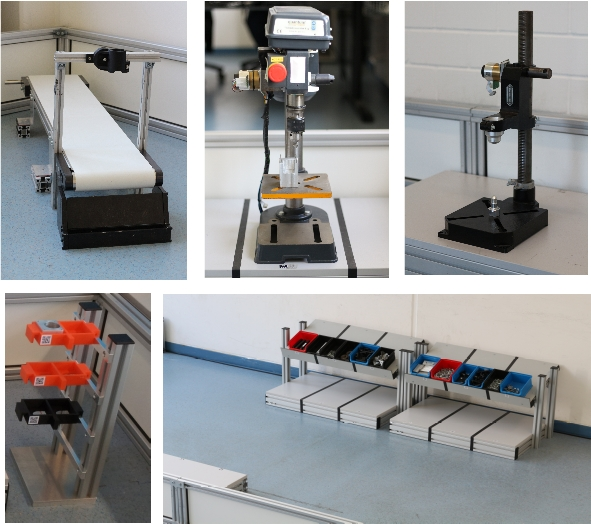
\includegraphics[width=14cm]{pics/atwork/arena_elements/AtWorkSpecsElements.jpg} 
 \end{center}
 \caption{\erlir arena elements and devices.}
 \label{fig:TaskRelatedObjects}
\end{figure}

\clearpage
\subsection{Variant}
	The arena is designed to be reconfigurable to accommodate different size and shape of the available space. 
	In this section, several variants of the environment are presented along with the required elements to build such variant.


\subsubsection{Prototype Variant}
	This variant is an early concept and a prototype of the reconfigurable and easy to transport arena from 2013. 
	The required elements are: 1. 3 x wall element 54; 2. 4 x wall element 80; 3. 6 x wall element 120 and 4. 7 x workstation.	The conveyor belt is the only device in the arena aside from the robot.
\begin{figure}[htb]
 \begin{center}
 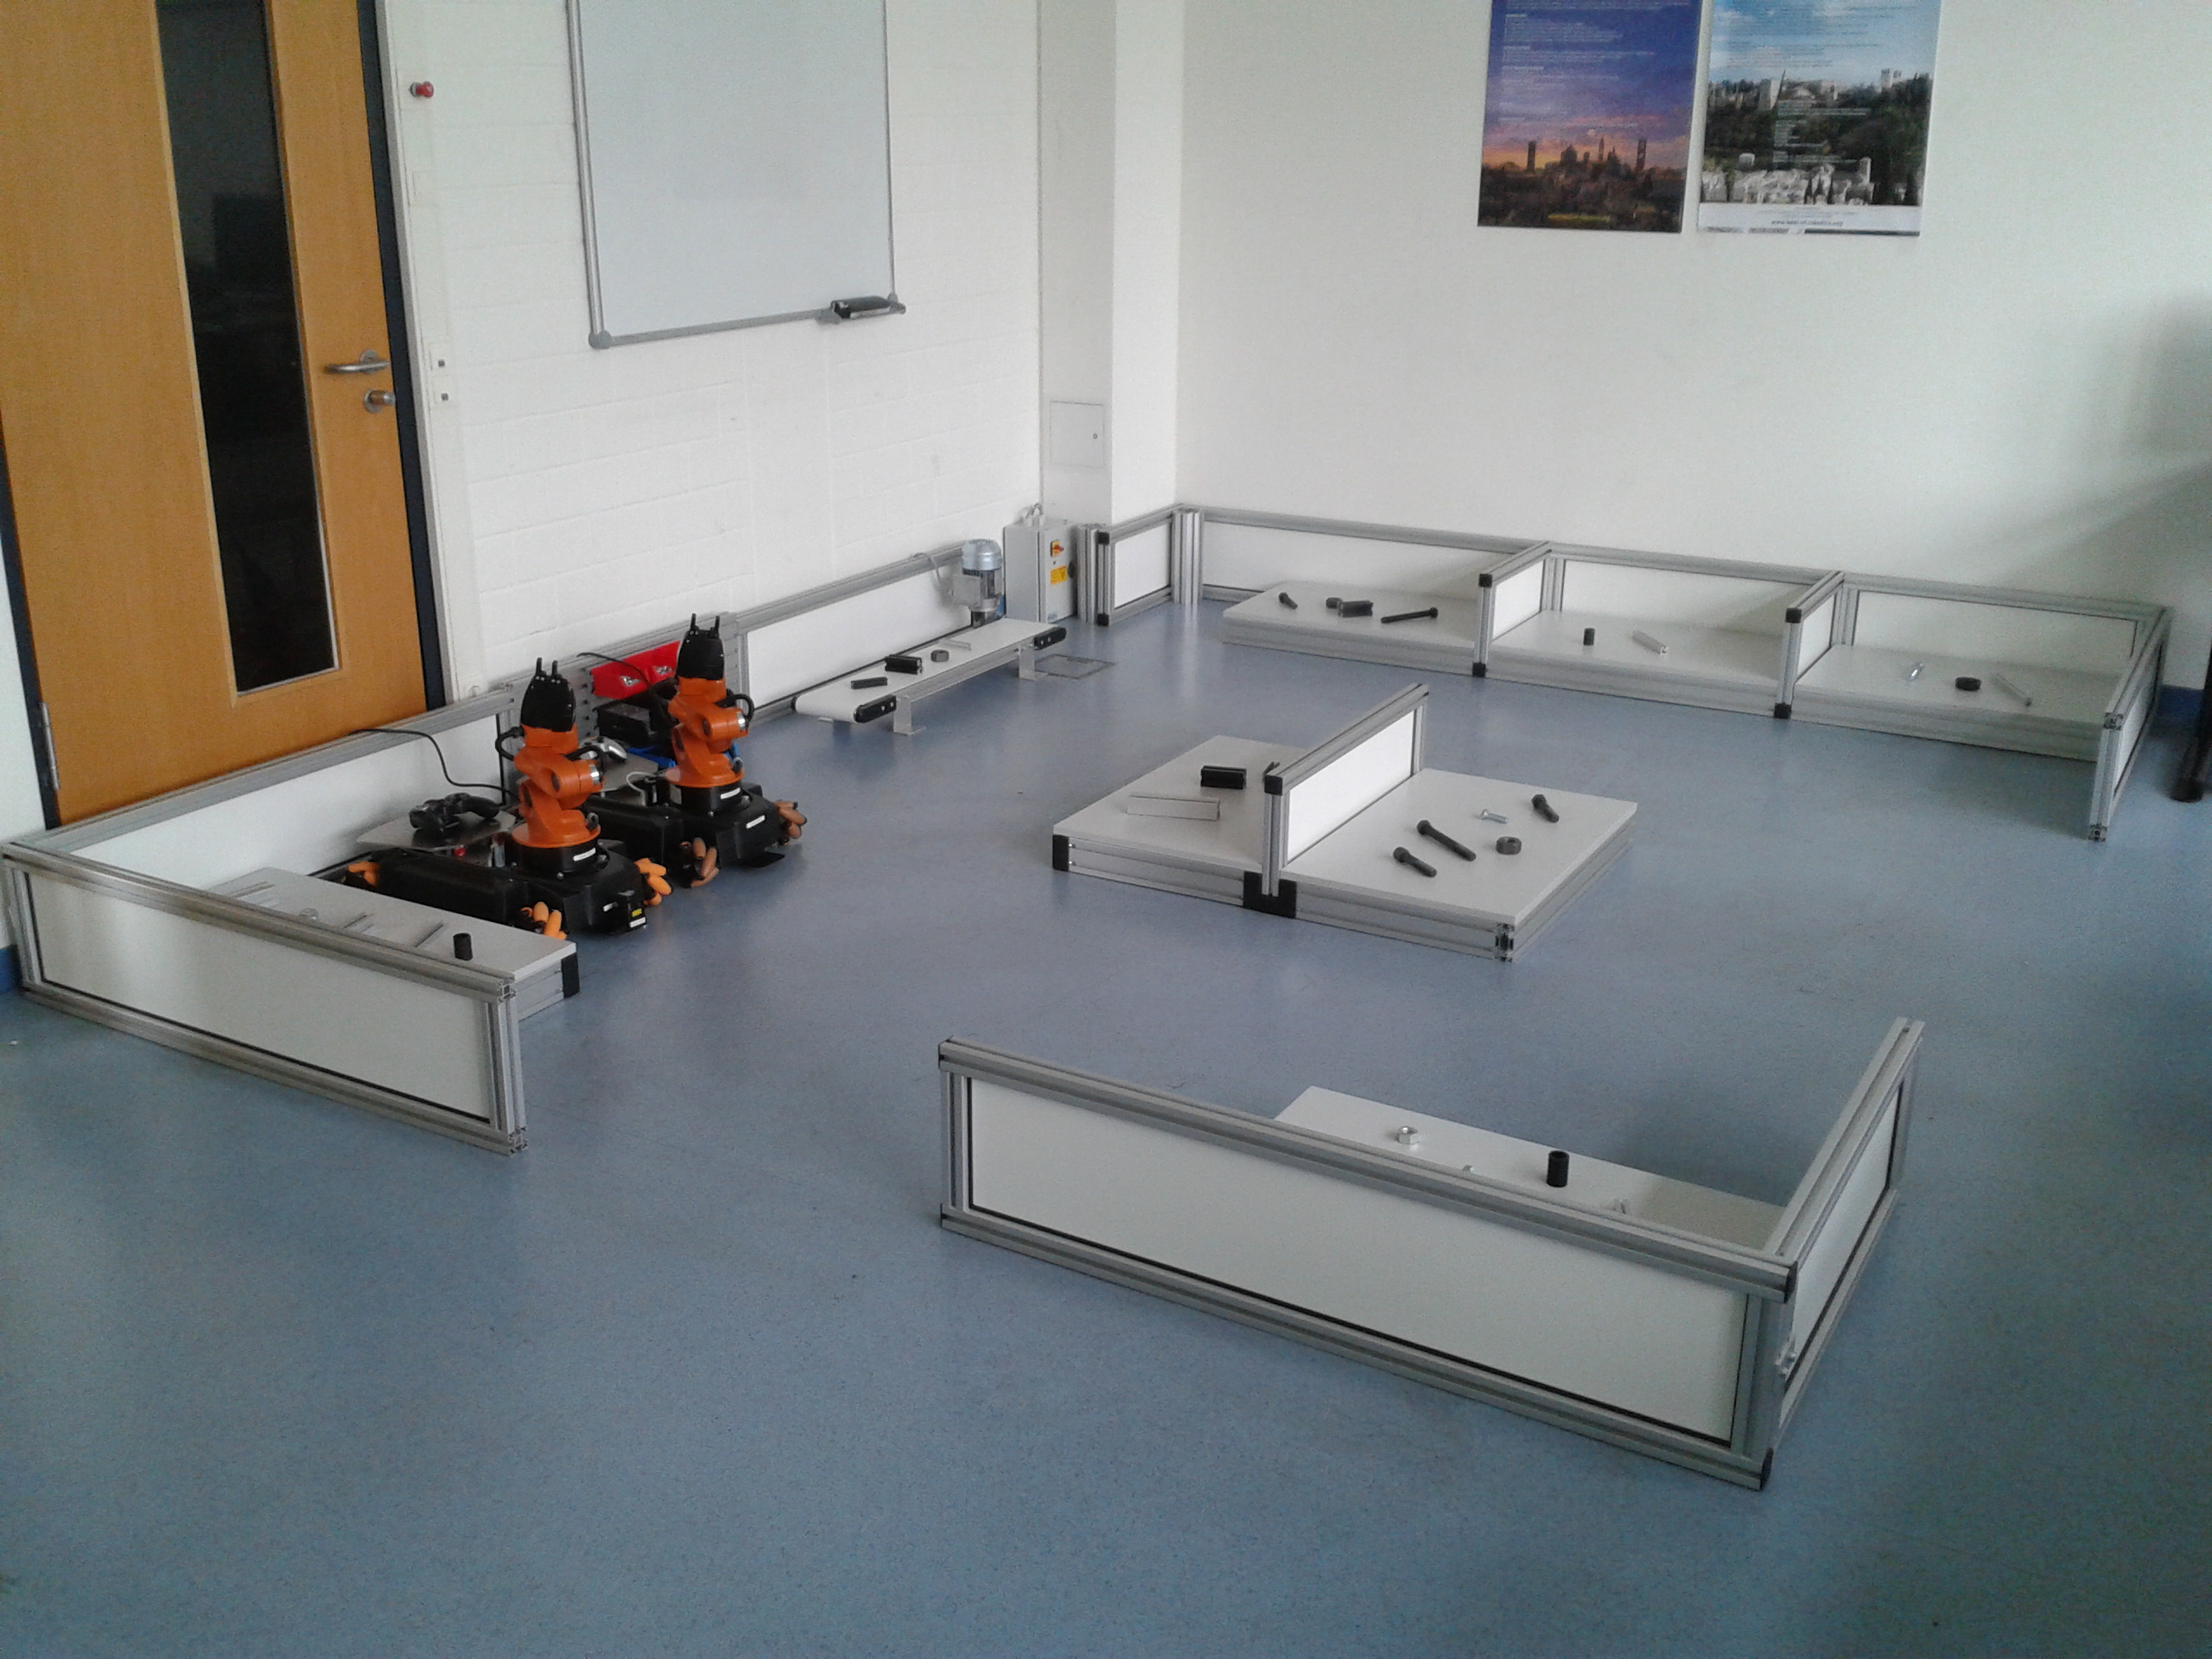
\includegraphics[width=12cm]{./fig/WorkArenaBRSU2013.jpg} 
 \caption{\roaw testbed 2013 variant}
  \label{fig:RoawTestBed2013} 

 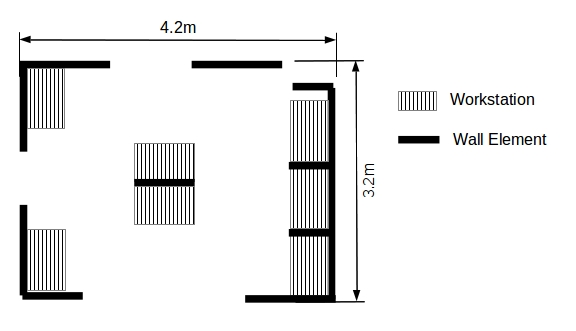
\includegraphics[width=12cm]{./fig/WorkArenaBRSU2013Dimension.jpg} 
 \caption{\roaw testbed 2013 variant dimension}
  \label{fig:RoawTestBed2013Dimension} 
   \end{center}
\end{figure}

\subsubsection{2014 Variant}
	This variant introduces: 1. shelves, 2. drilling machine, 3. force fitting machine and 4. assembly aid tray rack. The required elements are: 1. 3 x wall element 54; 2. 3 x wall element 80; 3. 4 x wall element 120; 4. 3 x workstation and 5. 2 x shelves set. 

\begin{figure}[htb]
 \begin{center}
 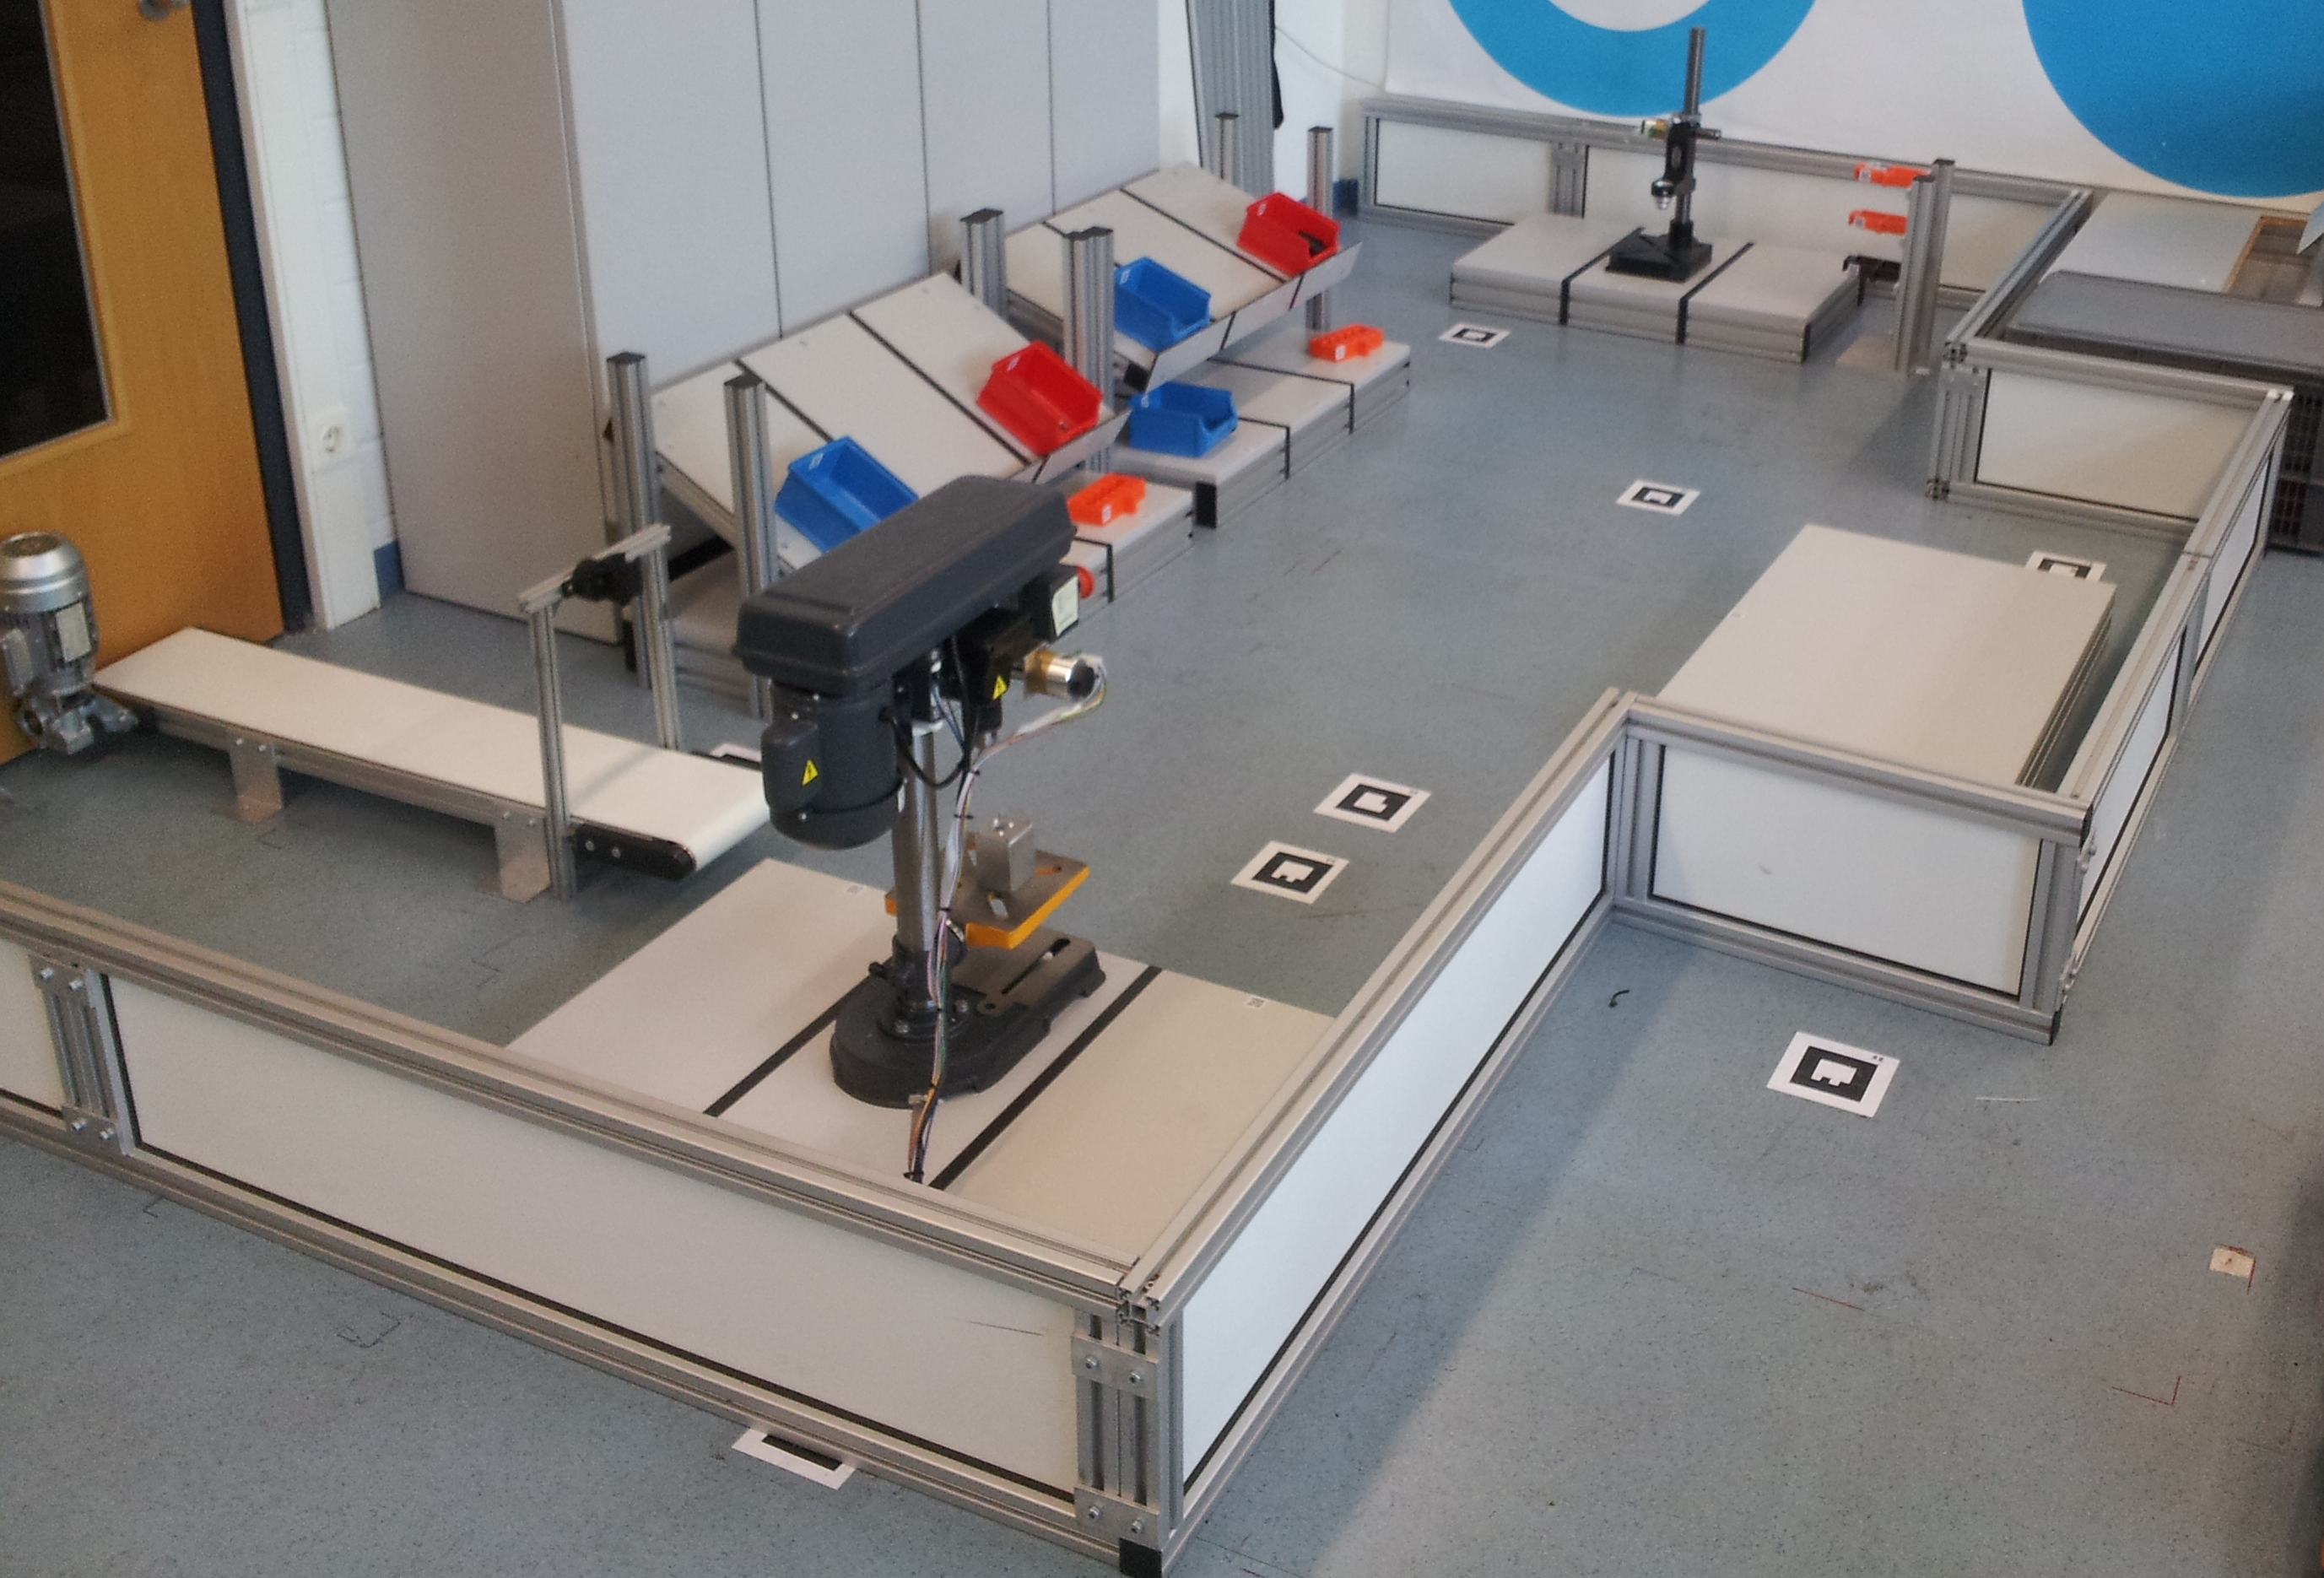
\includegraphics[width=14cm]{./fig/WorkArenaBRSU2014.jpg} 
 \caption{\roaw testbed 2014 variant}
 \label{fig:RoawTestBed2014} 

 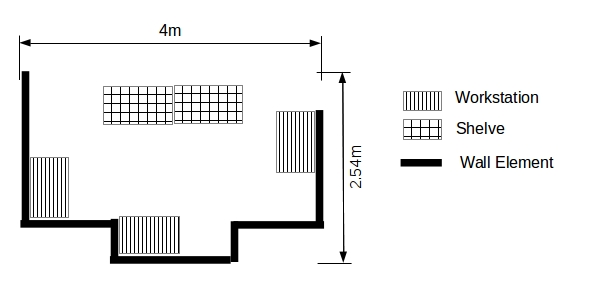
\includegraphics[width=14cm]{./fig/WorkArenaBRSU2014Dimension.jpg} 
 \end{center}
 \caption{\roaw testbed 2014 variant dimension}
  \label{fig:RoawTestBed2013Dimension} 
\end{figure}

\clearpage
\subsubsection{RoCKIn Variant}
	This variant is used for the RoCKIn project. The required elements for this variant are: 1. 2 x wall element 54; 2. 16 x wall element 80; 3. 6 x wall element 120; 4. 5 x workstation. and 5. 4 x shelves set.
	
\begin{figure}[htb]
 \begin{center}
 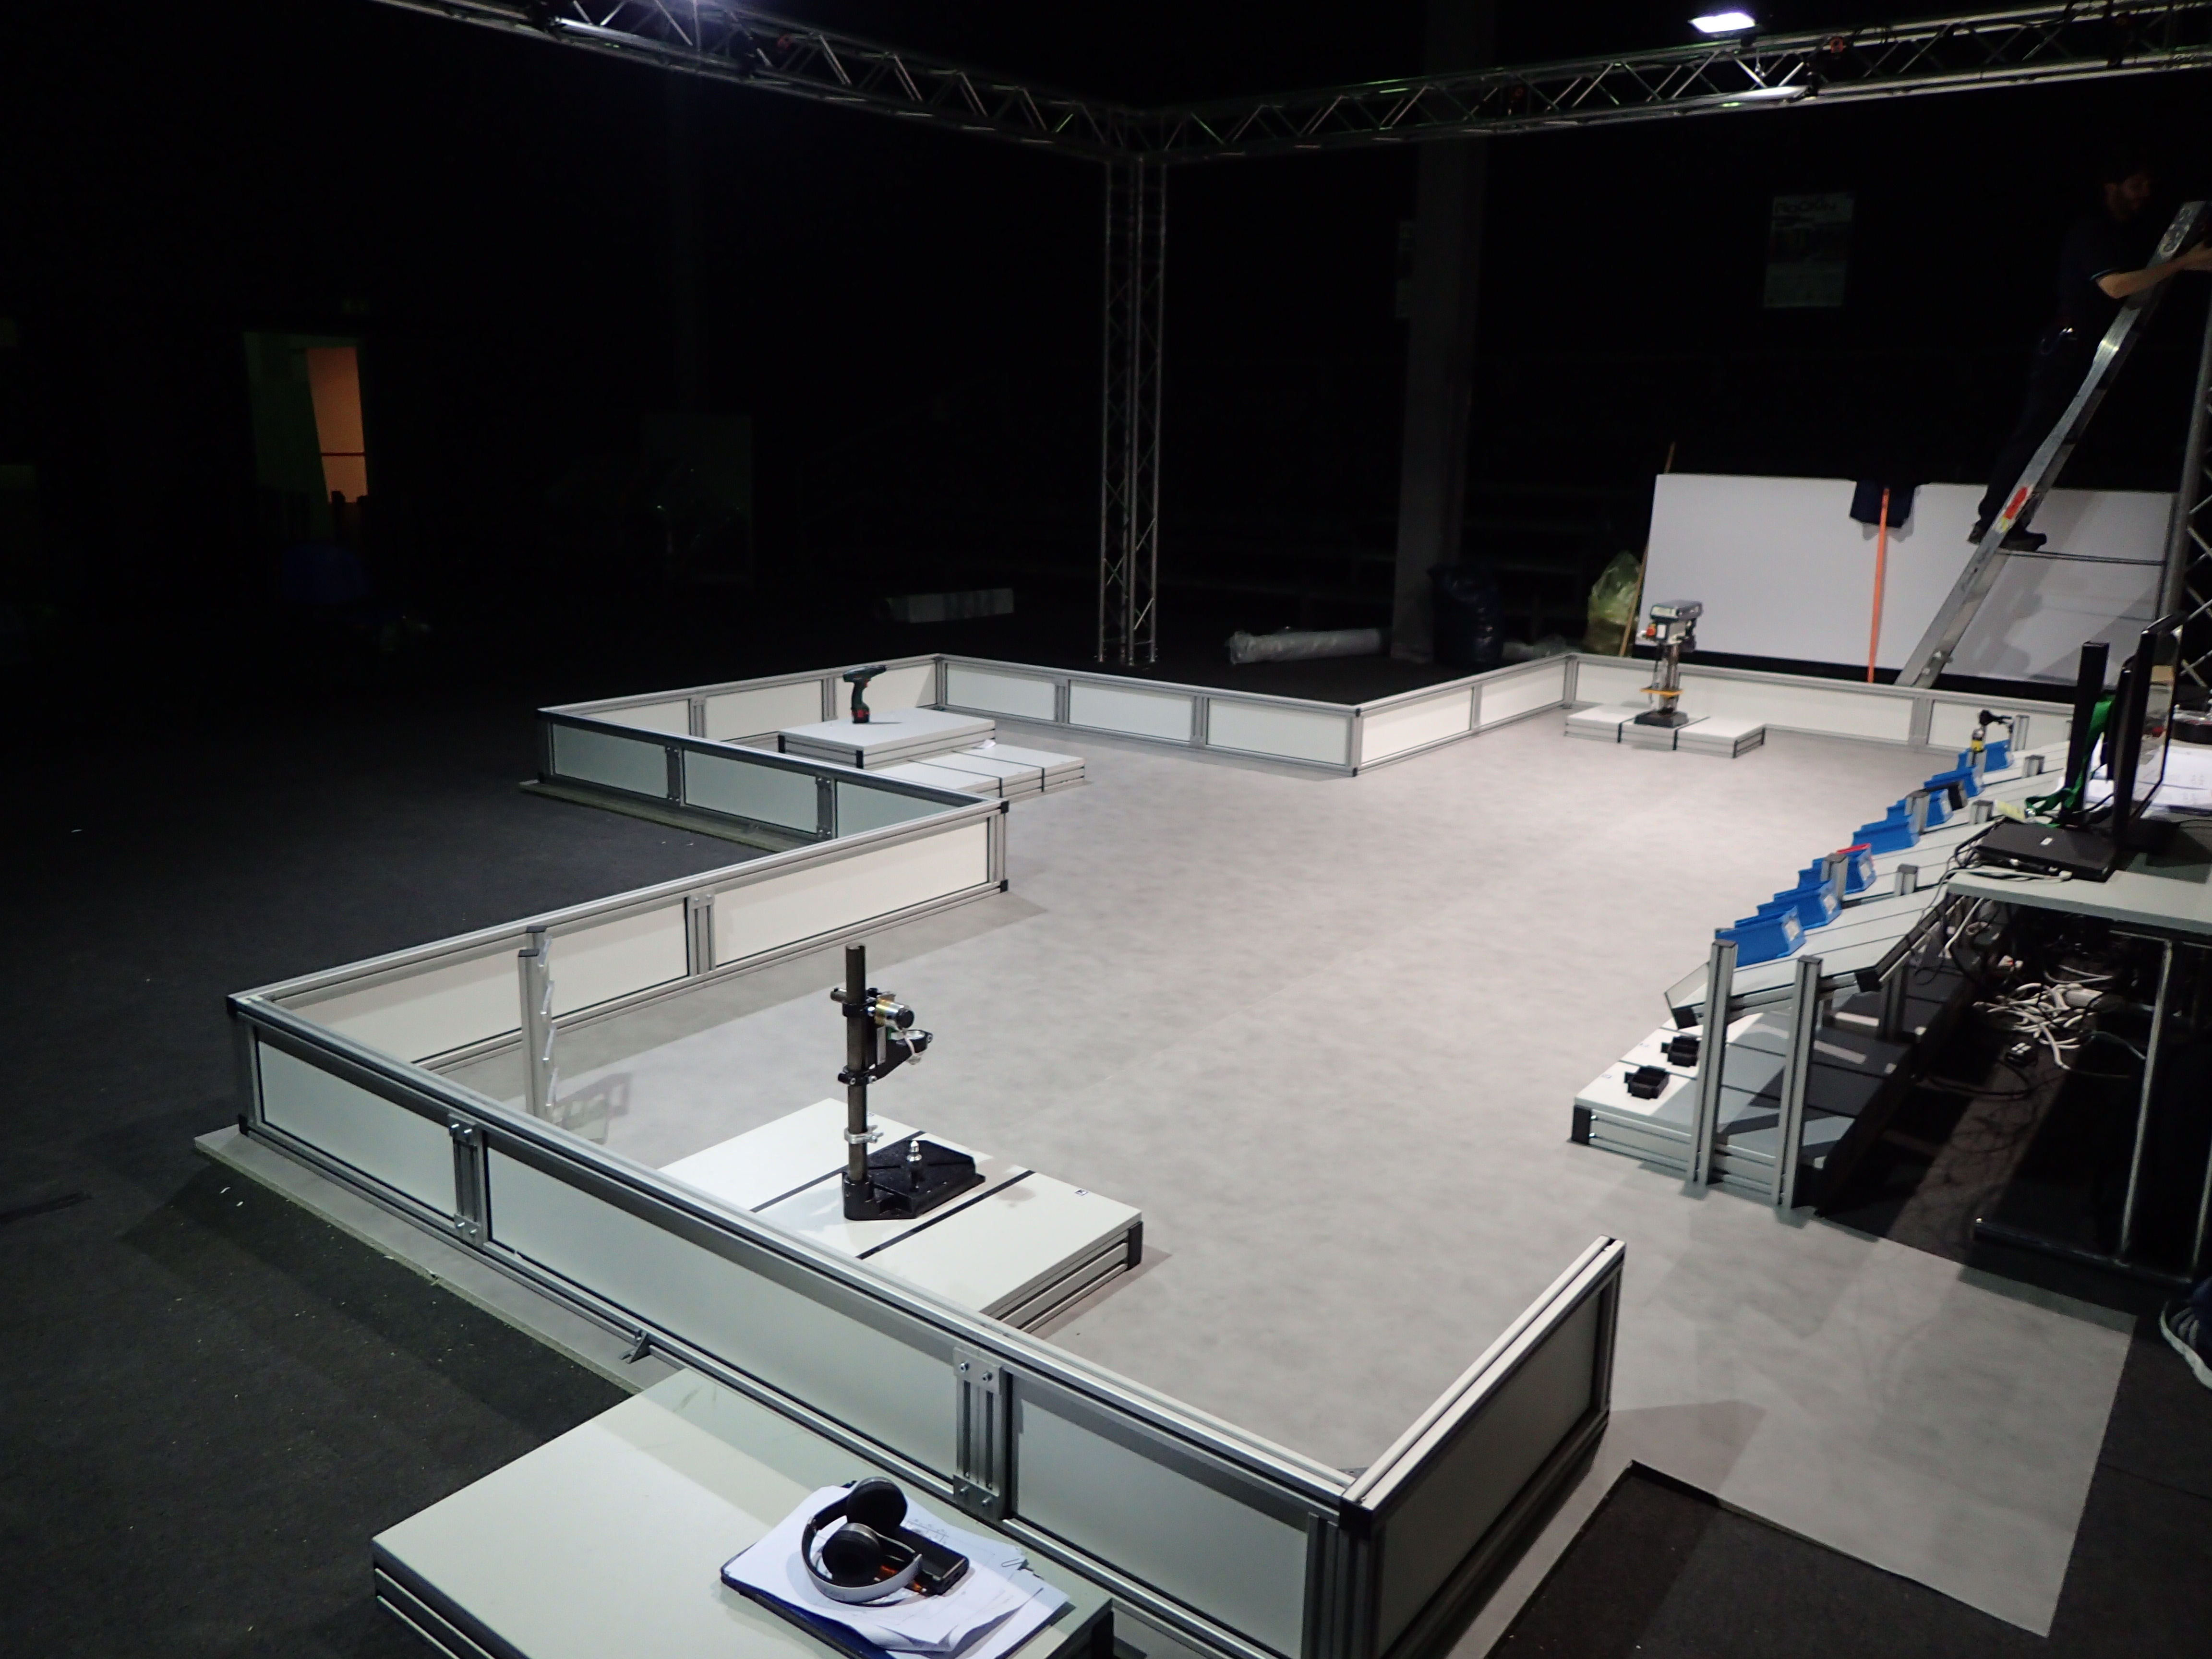
\includegraphics[width=10cm]{./fig/testbed/roaw_arena_lisbon.JPG} 
 \caption{\roaw 2015 competition testbed}
 \label{fig:RoawTestBed2014} 
 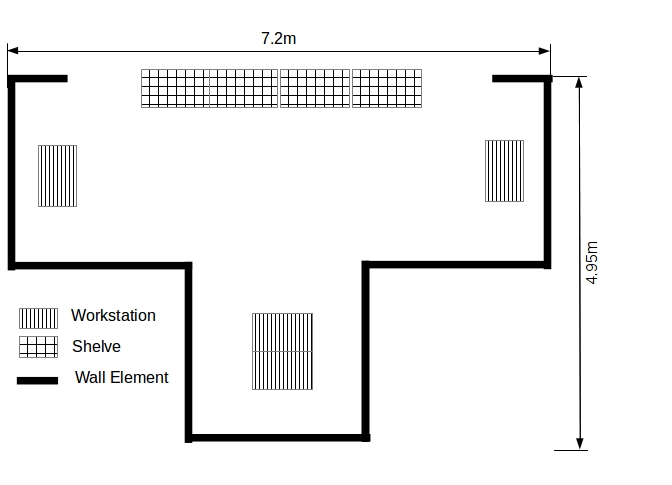
\includegraphics[width=12cm]{./fig/testbed/roaw_arena_lisbonDimension.jpg} 
 \end{center}
 \caption{\roaw 2015 competition testbed dimension}
  \label{fig:RoawTestBed2013Dimension} 
\end{figure}




